\section{Auswertung}
\label{sec:Auswertung}

\subsection{Bestimmung der Ausgleichsfunktionen}
Der gemessene Offset beträgt am Anfang der Messreihe $U_{0,Anfang} = \SI{0,0075}{\milli\volt}$ und am Ende $U_{0,Ende} = \SI{0,0088}{\milli\volt}$
Der Mittelwert beträgt dementsprechend $U_0 = \SI{0.00815}{\milli\volt}$.
$\Delta U = U_i - U_0$ ist demnach die wahre Spannung.
Die Temperatur im Raum betrug in etwa $T_0 = \SI{297,6}{\kelvin}$
Im Folgenden sind die Messdaten für matt, schwarz, glänzend und weiß in jener Reihenfolge aufgeführt:
\\
$Tabelle 1: T, U_1, delt U_1$
$Tabelle 2: T, U_2, delt U_2$
$Tabelle 3: T, U_3, delt U_3$
$Tabelle 4: T, U_4, delt U_4$
$[Werte nehmen aus Originaldaten]$
$[Alternativ: Ales in eine Tabelle mit 9 Spalten?]$
\\
Die Spannungen $\Delta U_i$ werden gegen die Differenz $T^4 - T_0^4$ in einem Diagramm aufgetragen.


Für die Ausgleichsrechnung wird ein linearer Zusammenhang der Form
\begin{equation}
  f(x) = mx + b
\end{equation}
erwartet.
Die Ausgleichsrechnung wird mit Hilfe der Gaußschen Methode der kleinsten Abweichungsquadrate durchgeführt.
Für die Steigung $m$ wird die Formel
\begin{equation}
  m = \frac{ n \sum_{i=1}^n x_i y_i - \sum_{i=1}^n x_i \sum_{i=1}^n y_i }{n\sum_{i=1}^n x_i^2 - ( \sum_{i=1}^n x_i )^2}
\end{equation}
verwendet. Dabei bezeichnet $n$ die Anzahl der Messungen, für $x_i$ und $y_i$ werden die jeweiligen Messwerte eingesetzt. Der Schnittpunkt mit der y-Achse wird durch
\begin{equation}
  b = \frac{ \sum_{i=1}^n x_i^2 \cdot \sum_{i=1}^n y_i - \sum_{i=1}^n x_i \cdot \sum_{i=1}^n x_i y_i}{n\sum_{i=1}^n x_i^2 - ( \sum_{i=1}^n x_i )^2}
\end{equation}

beschrieben.
Die Standardabweichung in y berechnet sich zu
\begin{equation}
  \sigma_y = \sqrt{ \frac {\sum_{i=1}^n (y_i-b-m \cdot x_i)}{n-2} }.
\end{equation}
Hieraus ergibt sich sofort
\begin{equation}
  \sigma_m = \sqrt{ \sigma_y^2 \frac{n}{n \sum_{i=1}^n x_i^2 - (\sum_{i=1}^n x)^2} }
\end{equation}
sowie
\begin{equation}
  \sigma_b = \sqrt{ \sigma_y^2 \frac{\sum_{i=1}^n x_i^2}{n \sum_{i=1}^n x_i^2 - (\sum_{i=1}^n x)^2} }
\end{equation}
für die Standardabweichungen in m und b.
Es ergeben sich für die Messreihen $U_1$ bis $U_4$ mit den Werten
\\
$Tabelle: m_1 +- Fehler, b_1 +- Fehler, usw.$
$[Werte nehmen aus Ui_Ausgleichsgerade.txt]$
$[Einheiten: b in Volt, m in Volt/Kelvin^4]$
\\
folgende Ausgleichsgeraden:
\begin{figure}[H]
  \centering
  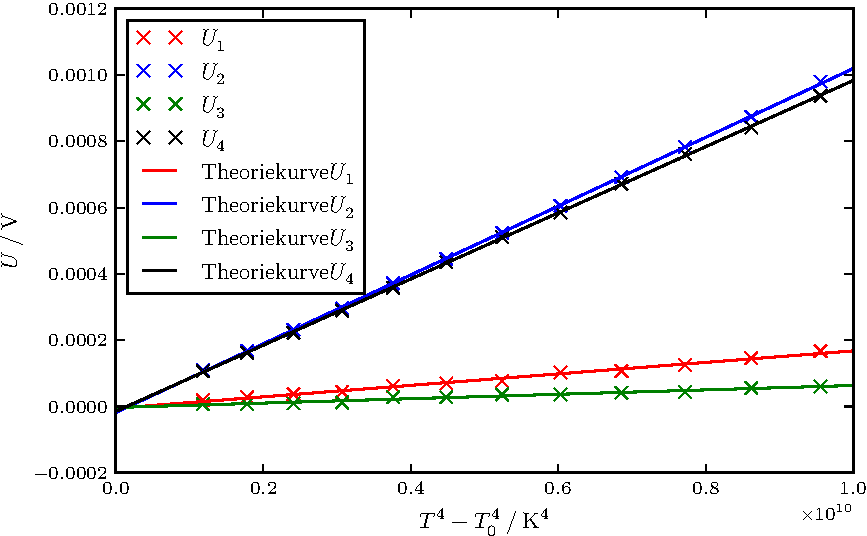
\includegraphics{plot.pdf}
  \caption{Plot.}
  \label{fig:plot}
\end{figure}

\cite{fehler}
\subsection{Bestimmung der Emissionsvermögen}
Um die Emissionsvermögen zu Bestimmen, werden die berechneten Steigungen der Ausgleichsfunktionen miteinander verglichen.
Die schwarze Oberfläche dient als Referenzwert und wird auf $\epsilon=1$ gesetzt.
Alle restlichen Emissionsverögen ergeben sich somit durch
\begin{equation}
  \epsilon_i = \frac{m_i}{m_s}
\end{equation}
wobei $m_s$ die Steigung der Ausgleichsgerade für $U_2$ ist.
Um den Fehler von $\epsilon_i$ zu bestimmen, wird die Gaußsche Fehlerfortpflanzung verwendet:
\begin{equation}
\increment{f} = \sqrt{\Bigl(\frac{\partial f}{\partial x_1}\increment{x_1}\Bigr)^2 + \Bigl(\frac{\partial f}{\partial x_2}\increment{x_2}\Bigr)^2 + \dotsc + \Bigl(\frac{\partial f}{\partial x_n}\increment{x_n}\Bigr)^2}
\end{equation}
Es folgt direkt
\begin{equation}
  \Delta\epsilon = \sqrt{ \Bigl( \frac{\partial \epsilon}{\partial m_i} \cdot \Delta m_i \Bigr)^2 +  \Bigl( \frac{\partial \epsilon}{\partial m_s} \cdot \Delta m_s  \Bigr)^2 } = \sqrt{ \frac{\Delta m_i ^2}{m_s^2} + \frac{m_i^2}{m_s^4} \Delta m_s^2 } .
\end{equation}
woraus sich für die Emissionsvermögen
\\
$Hier Werte aus Emissionsvermoegen.txt einfügen. Einheitenlos $
\\
\subsection{Strahlenintensität als Funktion des Abstandes}
